\documentclass[14pt,a4paper]{scrartcl}
\usepackage[utf8]{inputenc}
\usepackage[english,russian,ukrainian]{babel}
\usepackage{indentfirst}
\usepackage{misccorr}
\usepackage{graphicx}

\usepackage{cmap}
\usepackage{amsmath,amsfonts,amssymb,amsthm,mathtools}
\usepackage{icomma}
\usepackage{multirow}
\usepackage{geometry} \geometry{verbose,a4paper,tmargin=1cm,bmargin=2.5 cm,lmargin=2cm,rmargin=1cm}
\usepackage{euscript}
\usepackage{mathrsfs}
\usepackage{mathtext}
\usepackage{graphicx}
\usepackage{booktabs}
\usepackage{color}
\usepackage{rotating}
\usepackage{pdflscape}
\usepackage{floatrow}
\usepackage{subcaption}
\usepackage{calc}
\usepackage[table,xcdraw]{xcolor}
\linespread{1.3}
\setlength{\parindent}{5ex}


\begin{document}

\pagecolor{white}
\begin{titlepage}
  \begin{center}
    \large
    Національний технічний університет України \\ "Київський політехнічний інститут імені Ігоря Сікорського"
     
       
    Факультет Електроніки
     
    Кафедра мікроелектроніки
    \vfill
      
    \textsc{ЗВІТ}\\
     
    {\Large Про практичної роботи №2\\
      з дисципліни: «Твердотільна електроніка-2»\\[1cm]
      
    {\bf Розрахунок коефіцієнтів передачі біполярних та МДН-транзисторів}\\
    
    }
  \bigskip
\end{center}
\vfill
 
\newlength{\ML}
\settowidth{\ML}{«\underline{\hspace{0.4cm}}» \underline{\hspace{2cm}}}
\hfill
\begin{minipage}{1\textwidth}
Виконав:\\
Студент 3-го курсу \hspace{4cm} $\underset{\text{(підпис)}}{\underline{\hspace{0.2\textwidth}}}$  \hspace{1cm}Кузьмінський О.Р.\\
\vspace{1cm}

Перевірив: \hspace{6.1cm} $\underset{\text{(підпис)}}{\underline{\hspace{0.2\textwidth}}}$  \hspace{1 cm}Королевич Л.М.\\

\end{minipage}

\vfill

\begin{center}
2021
\end{center}
\end{titlepage}


\section{Біполярні транзистори}

\subsection{Схема зі спільною базою}
\begin{figure}[!h]\TopFloatBoxes\CenterFloatBoxes
\ffigbox{\caption{Схема включення зі спільною базою}}
{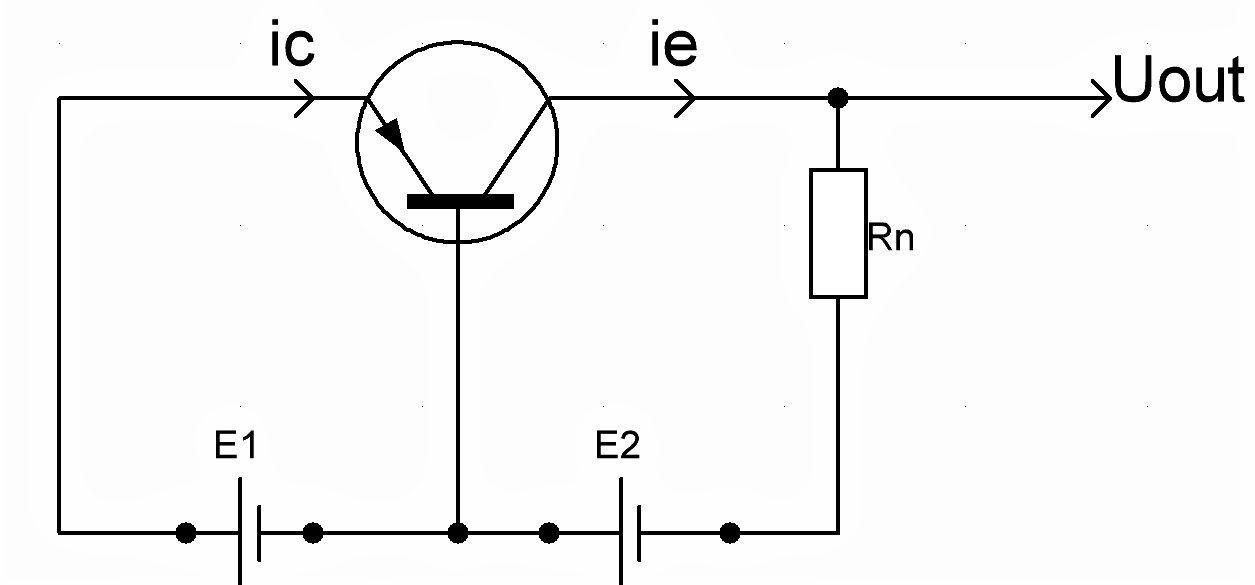
\includegraphics[width=0.7\textwidth]{combase}}
 \end{figure}

\begin{center}
$U_{out}=E_2-i_c\cdot{R_n}=i_c\cdot{R_c}$,\\[0.5cm]

$U_{in}=E_1=i_e\cdot{R_e}$,\\[0.5cm]

$K_U=\dfrac{U_{out}}{U_{in}}=\dfrac{i_c\cdot{R_c}}{i_e\cdot{R_e}}=\left|R_c>>R_e\right|\Rightarrow \boxed{K_U<<1}$\\[0.5cm]

$K_I=\dfrac{I_{out}}{I_{in}}=\dfrac{I_c}{I_e}=\left|I_c<I_e\right|\Rightarrow \boxed{K_I<1} (K_I\approx 0,95...0,99)$\\[0.5cm]
\end{center}
\medskip\hrule\medskip
\newpage

\subsection{Схема зі спільним колектором}
\begin{figure}[!h]\TopFloatBoxes\CenterFloatBoxes
\ffigbox{\caption{Схема включення зі спільним колектором}}
{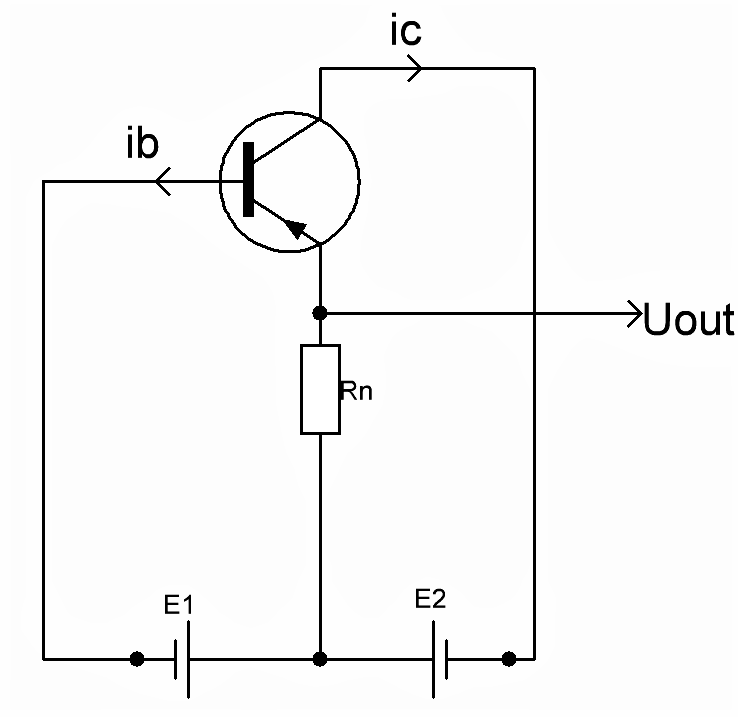
\includegraphics[width=0.5\textwidth]{comcol}}
 \end{figure}

\begin{center}
$U_{out}=-E_2+i_c\cdot{R_c}$\\[0.5cm]

$U_{in}=E_1=U_{out}+i_b\cdot{R_b}$\\[0.5cm]

$K_U=\dfrac{U_{out}}{U_{in}}=\dfrac{i_c\cdot{R_c}-E_2}{i_c\cdot{R_c}-E_2+i_b\cdot{R_b}}=\dfrac{U_{out}}{U_{out}+i_b\cdot{R_b}}\Rightarrow\boxed{K_U<1}$\\[0.5cm]

$K_I=\dfrac{I_{out}}{I_{in}}=\dfrac{I_e}{I_b}=\left|I_e>>I_b\right|\Rightarrow\boxed{K_I>>1}$
\end{center}
\medskip\hrule\medskip
\newpage
\subsection{Схема зі спільним емітером}
\begin{figure}[!h]\TopFloatBoxes\CenterFloatBoxes
\ffigbox{\caption{Схема включення зі спільним емітером}}
{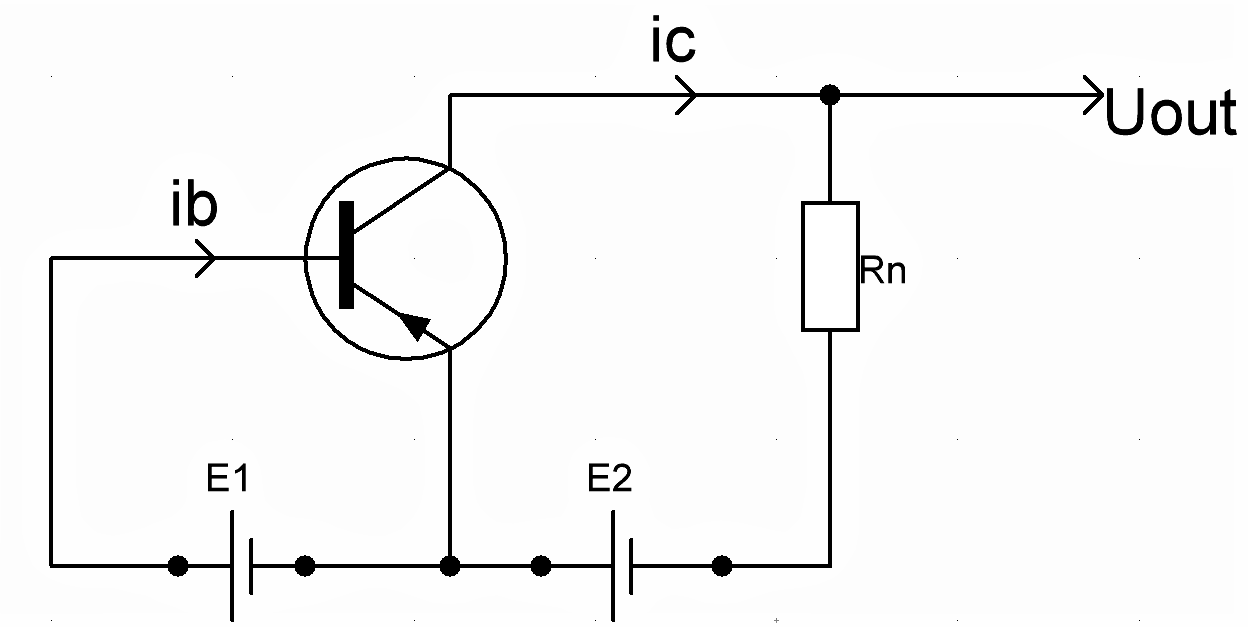
\includegraphics[width=0.7\textwidth]{comem}}
 \end{figure}

\begin{center}
$U_{out}=i_c\cdot{R_c}$\\[0.5cm]

$U_{in}=-i_b\cdot{R_b}$\\[0.5cm]

$K_U=\dfrac{U_{out}}{U_{in}}=-\dfrac{i_c\cdot{R_c}}{i_b\cdot{R_b}}=\left|R_c>>R_b\right|\Rightarrow\boxed{K_U>>1}$\\[0.5cm]

$K_I=\dfrac{I_{out}}{I_{in}}=\dfrac{I_c}{I_b}=\left|I_c>I_b\right|\Rightarrow\boxed{K_I>1}$
\end{center}

\medskip\hrule\medskip
\newpage


 \section{МДН-транзистори}




 \subsection{Схема зі спільним витоком}
\begin{figure}[!h]\TopFloatBoxes\CenterFloatBoxes
\ffigbox{\caption{Схема включення зі спільним витоком}}
{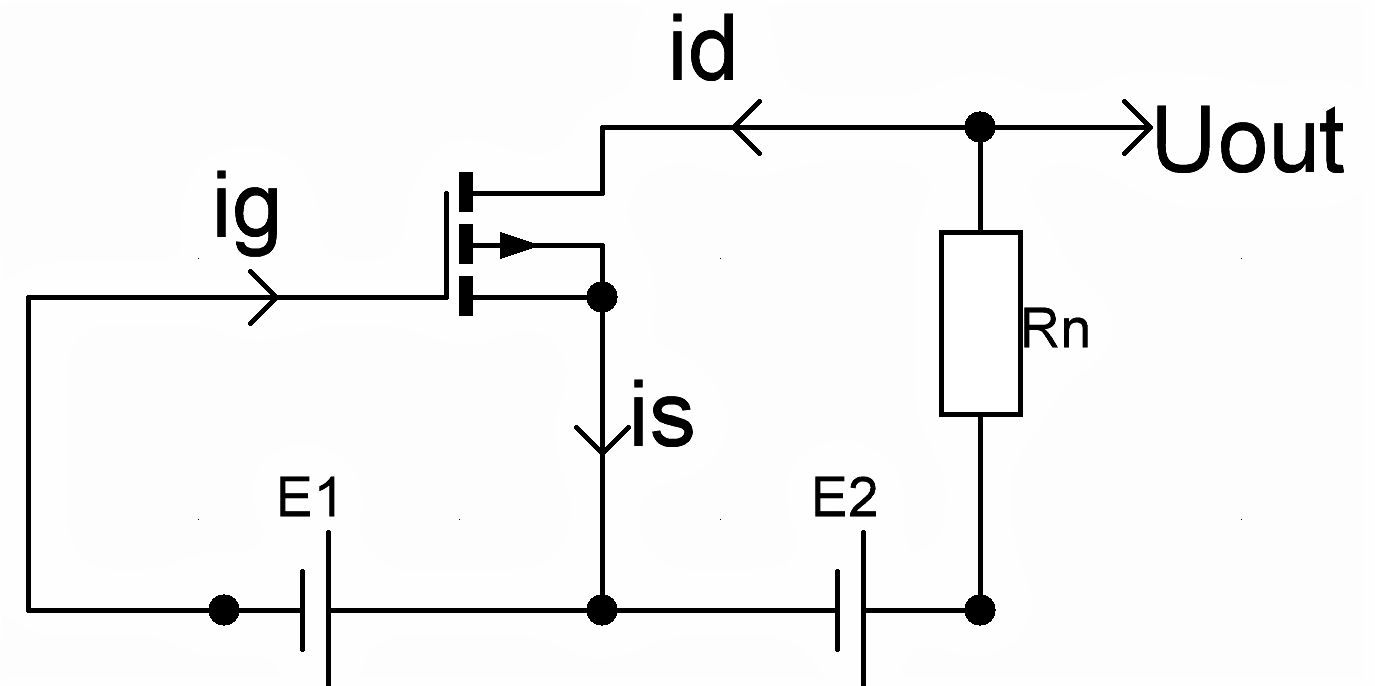
\includegraphics[width=0.7\textwidth]{comsource}}
 \end{figure}

\begin{center}
Затвор ізольований $\Rightarrow R_g>>1$\\[0.5cm]

$E_2>E_1$\\[0.5cm]

$U_{out}=i_d\cdot{R_d}-E_2$\\[0.5cm]

$U_{in}=-i_g\cdot{R_g}$\\[0.5cm]

$K_U=\dfrac{U_{out}}{U_{in}}=\dfrac{i_d\cdot{R_d}-E_2}{-i_g\cdot{R_g}}=\left|R_g>>1, i_g\rightarrow 0\right|\Rightarrow\boxed{K_U>>1}$.
\end{center}
\medskip\hrule\medskip
\newpage

\subsection{Схема зі спільним стоком}
\begin{figure}[!h]\TopFloatBoxes\CenterFloatBoxes
\ffigbox{\caption{Схема включення зі спільним стоком}}
{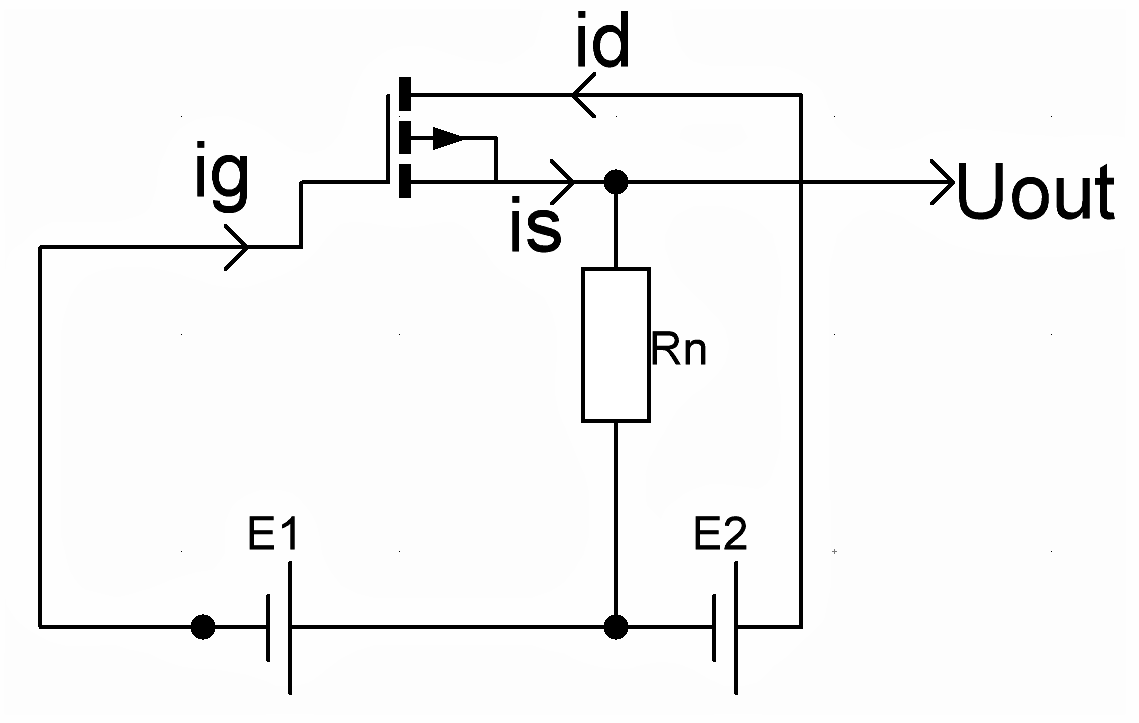
\includegraphics[width=0.7\textwidth]{comdrain}}
 \end{figure}

\begin{center}
$U_{out}=E_2-i_s\cdot{R_s}$\\[0.5cm]

$U_{in}=-R_n\cdot{i_s}-i_g\cdot{R_g}$\\[0.5cm]

$K_U=\dfrac{U_{out}}{U_{in}}=\dfrac{E_2-i_s\cdot{R_s}}{-R_n\cdot{i_s}-i_g\cdot{R_g}}\approx 1$
\end{center}
\medskip\hrule\medskip
\newpage

\subsection{Схема зі спільним затвором}
\begin{figure}[!h]\TopFloatBoxes\CenterFloatBoxes
\ffigbox{\caption{Схема включення зі спільним затвором}}
{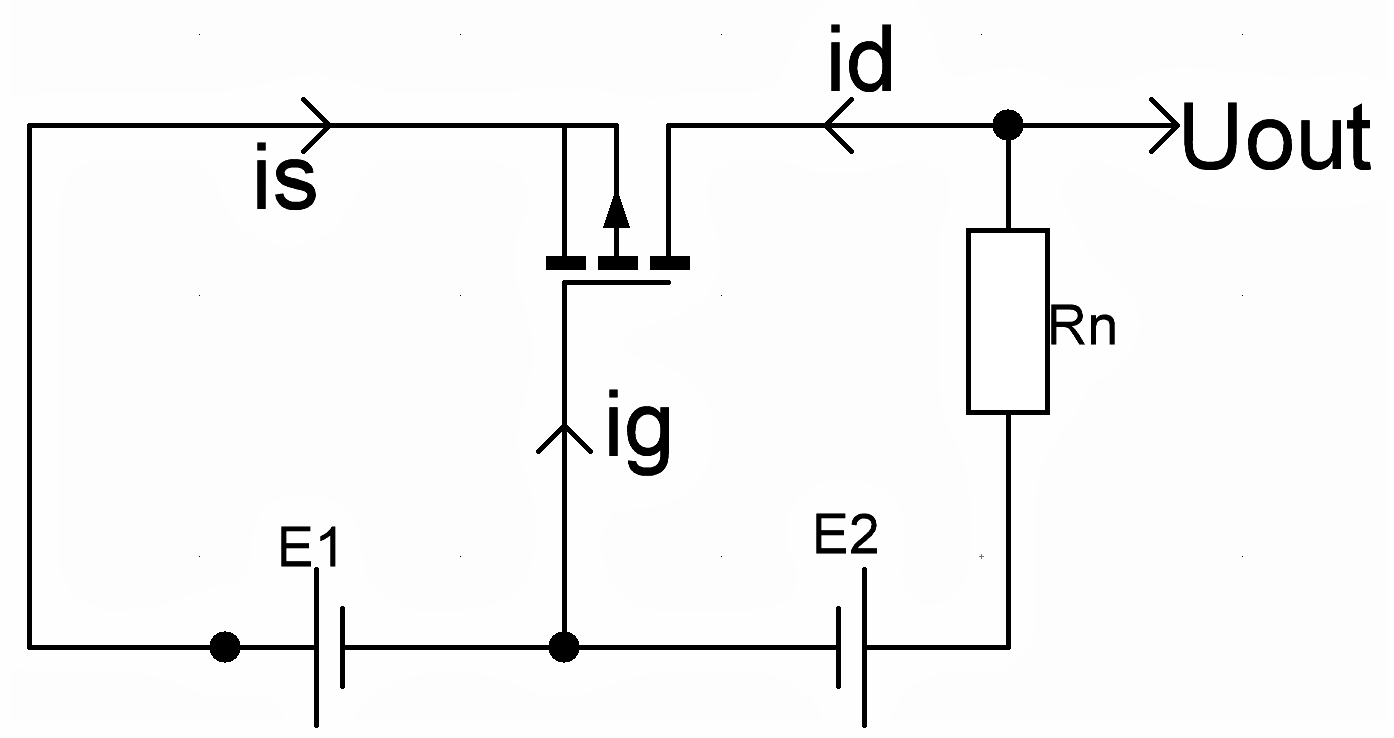
\includegraphics[width=0.7\textwidth]{comgate}}
 \end{figure}


\begin{center}
$U_{out}=i_d\cdot{R_n}+i_d\cdot{R_d}$\\[0.5cm]

$U_{in}=i_s\cdot{R_s}$\\[0.5cm]

$K_U=\dfrac{U_{out}}{U_{in}}=\dfrac{i_d\cdot{R_n}+i_d\cdot{R_d}}{i_s\cdot{R_s}}>1$
\end{center}









%\multirow{объединить Х строк}{ширина}{содержимое}
%\begin{tabular}{|p{6cm}|p{5cm}|p{5cm}|}
%\includegraphics[width=0.5\textwidth]{lablub}
%\medskip\hrule\medskip
%\multicolumn{2}{c|}{Диаметр}

\end{document}